\documentclass[12,]{article}
\usepackage[]{mathpazo}
\usepackage{setspace}
\setstretch{1.25}
\usepackage{amssymb,amsmath}
\usepackage{ifxetex,ifluatex}
\usepackage{fixltx2e} % provides \textsubscript
\ifnum 0\ifxetex 1\fi\ifluatex 1\fi=0 % if pdftex
  \usepackage[T1]{fontenc}
  \usepackage[utf8]{inputenc}
\else % if luatex or xelatex
  \ifxetex
    \usepackage{mathspec}
  \else
    \usepackage{fontspec}
  \fi
  \defaultfontfeatures{Ligatures=TeX,Scale=MatchLowercase}
\fi
% use upquote if available, for straight quotes in verbatim environments
\IfFileExists{upquote.sty}{\usepackage{upquote}}{}
% use microtype if available
\IfFileExists{microtype.sty}{%
\usepackage[]{microtype}
\UseMicrotypeSet[protrusion]{basicmath} % disable protrusion for tt fonts
}{}
\PassOptionsToPackage{hyphens}{url} % url is loaded by hyperref
\usepackage[unicode=true]{hyperref}
\hypersetup{
            pdftitle={Graph Gallery},
            pdfauthor={Vinter Capital},
            pdfborder={0 0 0},
            breaklinks=true}
\urlstyle{same}  % don't use monospace font for urls
\usepackage{graphicx,grffile}
\makeatletter
\def\maxwidth{\ifdim\Gin@nat@width>\linewidth\linewidth\else\Gin@nat@width\fi}
\def\maxheight{\ifdim\Gin@nat@height>\textheight\textheight\else\Gin@nat@height\fi}
\makeatother
% Scale images if necessary, so that they will not overflow the page
% margins by default, and it is still possible to overwrite the defaults
% using explicit options in \includegraphics[width, height, ...]{}
\setkeys{Gin}{width=\maxwidth,height=\maxheight,keepaspectratio}
\IfFileExists{parskip.sty}{%
\usepackage{parskip}
}{% else
\setlength{\parindent}{0pt}
\setlength{\parskip}{6pt plus 2pt minus 1pt}
}
\setlength{\emergencystretch}{3em}  % prevent overfull lines
\providecommand{\tightlist}{%
  \setlength{\itemsep}{0pt}\setlength{\parskip}{0pt}}
\setcounter{secnumdepth}{5}
% Redefines (sub)paragraphs to behave more like sections
\ifx\paragraph\undefined\else
\let\oldparagraph\paragraph
\renewcommand{\paragraph}[1]{\oldparagraph{#1}\mbox{}}
\fi
\ifx\subparagraph\undefined\else
\let\oldsubparagraph\subparagraph
\renewcommand{\subparagraph}[1]{\oldsubparagraph{#1}\mbox{}}
\fi

% set default figure placement to htbp
\makeatletter
\def\fps@figure{htbp}
\makeatother


\title{Graph Gallery}
\author{Vinter Capital}
\date{}

\begin{document}
\maketitle

{
\setcounter{tocdepth}{2}
\tableofcontents
}
\begin{verbatim}
\graphicspath{{./Figures/}}
\end{verbatim}

\section{test}\label{test}

caption in many pages

\section{TODO}\label{todo}

make a python script that send to terminal, firstly .md to .tex secondly
.tex to .pdf

this section describes what i need to do.

there are errors in the files. you cannot point to
/jl/Documents/crinfu/output because some are wrong e.g.~turnover\_1 is
not at all what it should be. solve this by running code in pycharm on
clinux to get the correct output.

\section{Theory}\label{theory}

For those accustomed to time series analysis and reading financial
charts, this section is not needed. For everyone else, this section
provides a point of reference - similar to a glossary.

\subsection{Prices}\label{prices}

\subsection{Returns}\label{returns}

\subsection{Weights}\label{weights}

\subsection{Volatility}\label{volatility}

\subsection{Correlation}\label{correlation}

\subsection{Autocorrelation}\label{autocorrelation}

\subsection{Rolling windowkeyboard}\label{rolling-windowkeyboard}

todo insert plot from my su thesis

If you have data from day 1 to day 1000, you can split it up into
rolling time period of 100 days so that the first windows is day 1 to
100, the second window is day 2 to 101, and so on.

Using these windows, each of which contain 100 days, we can then compute
a statistic such as the mean price for each window. By plotting the mean
price on the y-axis and the window's end date on the x-axis, we can see
how the mean changed depending on the data that is used.

Another feature of rolling windows is to smooth data that is volatile,
so that the lines in a graph are smoother.

\subsection{Weight caps and floors}\label{weight-caps-and-floors}

With a cap, the weight of asset get modified from
\texttt{w\textquotesingle{}} to
\texttt{w\ =\ max(w\textquotesingle{},\ weight\ cap)}. With a weight
floor, the weight of asset get modified from
\texttt{w\textquotesingle{}} to
\texttt{w\ =\ min(w\textquotesingle{},\ weight\ floor)}.

A weight cap can reduce the weight in large assets, and a weight floors
can increase the weight in small assets. Large and small, in tis
contect, refer to the market capitalization of the asset.

When a weight cap is imposed, the ``removed'' weights must be
redistributed so that the weights sum to 100\%. For example, if BTC has
weight 55\% according to its market capitalization, and a basket has a
weight cap of 30\%, then 25\% weight is removed from the basked and that
must be redistributed to other assets somehow. Vinter Capital achieve
this by taking the removed weight (e.g.~25\%) and allocating it to all
other assets in the basket, according to their previous weight.

The assets whose weights change when a weight floor is imposed get an
increased weight. When a weight floor is imposed, the ``added'' weights
must be taken from somewhere so that the weights sum to 100\%. For
example, if the tenth asset has a market capitalization so that its
weight is 0.6\% and we impose a weight floor of 1\% then the extra 0.4\%
has to come from somewhere - otherwise the index weights sum to 100.4\%.
Vinter Capital achieve this by stealing the added weight (e.g.~0.4\%)
from all other assets in the basket, except those who have been affected
from the cap.

\section{Files}\label{files}

\begin{verbatim}
/home/he2/Documents/crinfu/output/vcc/vol/volfr_vcc_bsk1_smooth20.png
/home/he2/Documents/crinfu/output/vcc/vol/volfr_vcc_smooth20.png
/home/he2/Documents/crinfu/output/vcc/vol/vol_vcc_bsk1_smooth20.png
/home/he2/Documents/crinfu/output/vcc/vol/vol_vcc_smooth20.png

/home/he2/Documents/crinfu/output/vcc/ret/price-fund_vs_coins.png
/home/he2/Documents/crinfu/output/vcc/ret/pri_portfolios.png
/home/he2/Documents/crinfu/output/vcc/ret/pri_portfolios_2.png
/home/he2/Documents/crinfu/output/vcc/ret/pri_t5.png
/home/he2/Documents/crinfu/output/vcc/ret/pri_tkr3_market.png
/home/he2/Documents/crinfu/output/vcc/ret/retvol_scatter_text.png
/home/he2/Documents/crinfu/output/vcc/ret/total_marketcap.png
/home/he2/Documents/crinfu/output/vcc/ret/vcc-rollcorr-t5_smooth20.png
/home/he2/Documents/crinfu/output/vcc/ret/vcc-rollcorr-t10_smooth20.png
/home/he2/Documents/crinfu/output/vcc/ret/woobull.png
/home/he2/Documents/crinfu/output/vcc/ret/pri_portfolios.csv

/home/he2/Documents/crinfu/output/vcc/mca/mca_vcc.png
/home/he2/Documents/crinfu/output/vcc/mca/mca_vcc_bsk1.png

/home/he2/Documents/crinfu/output/bsk/wei/capsweight floors_effect_1_alts.png
/home/he2/Documents/crinfu/output/bsk/wei/capsweight floors_effect_1_BTC.png
/home/he2/Documents/crinfu/output/bsk/wei/coinswitches1.png
/home/he2/Documents/crinfu/output/bsk/wei/coinswitches1minus4.png
/home/he2/Documents/crinfu/output/bsk/wei/coinswitches4.png
/home/he2/Documents/crinfu/output/bsk/wei/coinswitches8.png
/home/he2/Documents/crinfu/output/bsk/wei/mcafr_bsk1bsk4_smooth20.png
/home/he2/Documents/crinfu/output/bsk/wei/smoothing_w1.png
/home/he2/Documents/crinfu/output/bsk/wei/turnover_1.png
/home/he2/Documents/crinfu/output/bsk/wei/turnover_2.png
/home/he2/Documents/crinfu/output/bsk/wei/volume_5vs10_1.png
/home/he2/Documents/crinfu/output/bsk/wei/w1_alts.png
/home/he2/Documents/crinfu/output/bsk/wei/w1_area.png
/home/he2/Documents/crinfu/output/bsk/wei/w4-1m_alts.png
/home/he2/Documents/crinfu/output/bsk/wei/w4_alts.png
/home/he2/Documents/crinfu/output/bsk/wei/w4_area.png
/home/he2/Documents/crinfu/output/bsk/wei/w4-w1_area.png
/home/he2/Documents/crinfu/output/bsk/wei/wd1_tkr_insouts_mostwei.png
/home/he2/Documents/crinfu/output/bsk/wei/coinswitches_bsk1.txt
/home/he2/Documents/crinfu/output/bsk/wei/coinswitches_bsk1_minus_bsk4.txt
/home/he2/Documents/crinfu/output/bsk/wei/member_sum_wei_t5-wm-rm.txt
/home/he2/Documents/crinfu/output/bsk/wei/member_sum_wei_t10-wm-rm.txt
/home/he2/Documents/crinfu/output/bsk/wei/nrof_coinsw_w1.csv
/home/he2/Documents/crinfu/output/bsk/wei/smoothing_1.csv
/home/he2/Documents/crinfu/output/bsk/wei/tkr_insouts_mostwei_sum.csv
/home/he2/Documents/crinfu/output/bsk/wei/w4_minusw_1m_mean.csv
/home/he2/Documents/crinfu/output/bsk/wei/wd_mean.txt
/home/he2/Documents/crinfu/output/bsk/wei/wei_mthly_t5-wm-rm.csv
/home/he2/Documents/crinfu/output/bsk/wei/wei_mthly_t10-wm-rm.csv
/home/he2/Documents/crinfu/output/bsk/wei/w smooth minus w raw, abs(mean()).csv

/home/he2/Documents/crinfu/output/bsk/ret/ACF_bsk1.png
/home/he2/Documents/crinfu/output/bsk/ret/ACF_btc.png
/home/he2/Documents/crinfu/output/bsk/ret/bsk-rollcorr-1.png
/home/he2/Documents/crinfu/output/bsk/ret/contribution_bsk1.png
/home/he2/Documents/crinfu/output/bsk/ret/contribution_bsk4.png
/home/he2/Documents/crinfu/output/bsk/ret/qqplot_BTC.png
/home/he2/Documents/crinfu/output/bsk/ret/qqplot_market.png
/home/he2/Documents/crinfu/output/bsk/ret/ret_dens_market.png
/home/he2/Documents/crinfu/output/bsk/ret/retmat1_box.png
/home/he2/Documents/crinfu/output/bsk/ret/retmat1_rollbeta.png
/home/he2/Documents/crinfu/output/bsk/ret/retmat1_rolling_sharpe_1.png
/home/he2/Documents/crinfu/output/bsk/ret/retmat1_rollvol.png
/home/he2/Documents/crinfu/output/bsk/ret/retmat1_beta.csv
/home/he2/Documents/crinfu/output/bsk/ret/retmat1_descr_interval.csv
/home/he2/Documents/crinfu/output/bsk/ret/retmat1_risk.csv
/home/he2/Documents/crinfu/output/bsk/ret/retmat1_yearly_mean.csv
/home/he2/Documents/crinfu/output/bsk/ret/retmat1_yearly_vol.csv
\end{verbatim}

\section{Description of digital
assets}\label{description-of-digital-assets}

\subsection{Prices}\label{prices-1}

pri\_t5

\subsection{Market cap}\label{market-cap}

total\_marketcap

\subsection{Returns}\label{returns-1}

qqplot\_market qqplot\_BTC

\section{Description and comparison of
indices}\label{description-and-comparison-of-indices}

\subsection{Prices}\label{prices-2}

\subsection{Market cap}\label{market-cap-1}

\subsection{Returns}\label{returns-2}

contribution\_bsk1 contribution\_bsk4

retmat1\_box

\subsection{Risk \& returns}\label{risk-returns}

retvol\_scatter\_text

\subsection{Risk \& return}\label{risk-return}

retmat1\_rollvol

retmat1\_rolling\_sharpe\_1

retmat1\_rollbeta

\subsection{Weights}\label{weights-1}

\subsubsection{caps and floors}\label{caps-and-floors}

The defintion for caps and floors are found in the theory section.

\begin{figure}
\centering
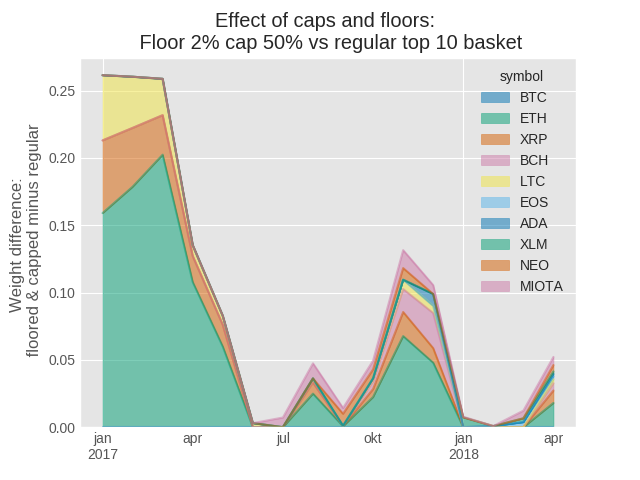
\includegraphics{/home/he2/Documents/crinfu/output/bsk/wei/capsfloors_effect_1_alts.png}
\caption{Stacked area chart of weight difference between on one hand a
regular market capitalization weighted top 10 basket, versus on the
other hand imposing weight caps and floors. This graph answer the
question: How does the weight in each asset change when weight caps and
floors are imposed? On the y-axis we see how large this effect is. The
colors represent an asset - clearly ETH is most affected, followed by
XRP and LTC. The reason for this is the historical dominance of BTC well
above 50\%. With a cap of 50\% some weight is taken from BTC and
allocated to the other nine assets, in accordance with their previous
weight. With a floor of 2\% the smallest assets get a boost in their
weight, especially the ninth and tenth asset. In relative terms, changes
can be vast (it can go from 0.2\% to 2\% which is a 10x increase) but in
absolute terms the changes are small and are thus not seen clearly in
this graph.}
\end{figure}

A lower cap value, e.g.~30\% instead of 50\%, decrease the weight in BTC
even more - this in turn increases t the weight in alt coins since the
weights must sum to one.

\subsubsection{some files}\label{some-files}

w1\_alts.png w4\_alts.png

w4-1m\_alts.png w1\_area.png

\subsubsection{fraction of market cap}\label{fraction-of-market-cap}

This graph answer the question:

\begin{quote}
How much closer to the ``total'' market is a top 10 compared to a top 5
basket?
\end{quote}

The fraction of total market capitalzation for a certain basket is
defined as the market capitalzation of the assets in the basket, divided
by the total market capitalzation. (To get smoother lines a 20 day mean
is imposed in the graph.) In order to be logically consistent and
practical, we define the total market as a basket with 200 assets
weighted by market capitalzation.

\begin{figure}
\centering
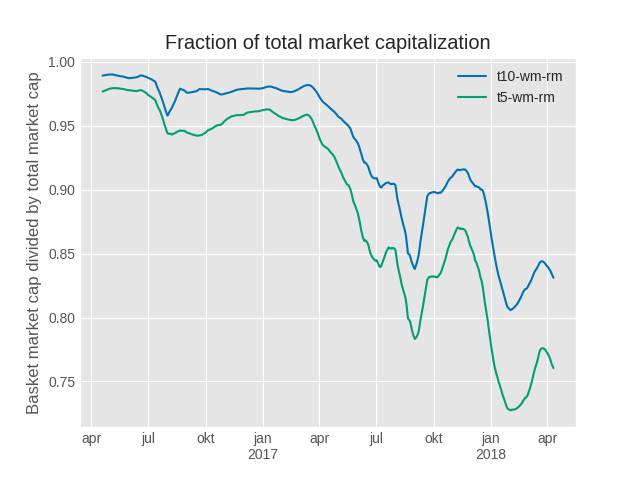
\includegraphics{/home/he2/Documents/crinfu/output/bsk/wei/mcafr_bsk1bsk4_smooth20.png}
\caption{A top 10 basket capture around 90\% of the total market
capitalization, and a top 5 basket slightly less. Over time, the
fraction is decreasing, indicating that the coins with a market
capitalzation ranked below 11 are growing in size relative to the top
10. In the future, a top 20 or top 50 index might be needed to capture
the market.}
\end{figure}

\begin{quote}
stylish question: is it better to put everything in the caption, or is
it better to
\end{quote}

\subsubsection{Turnover on rebalancing
date}\label{turnover-on-rebalancing-date}

\begin{quote}
What is the turnover in small assets?
\end{quote}

\begin{figure}
\centering
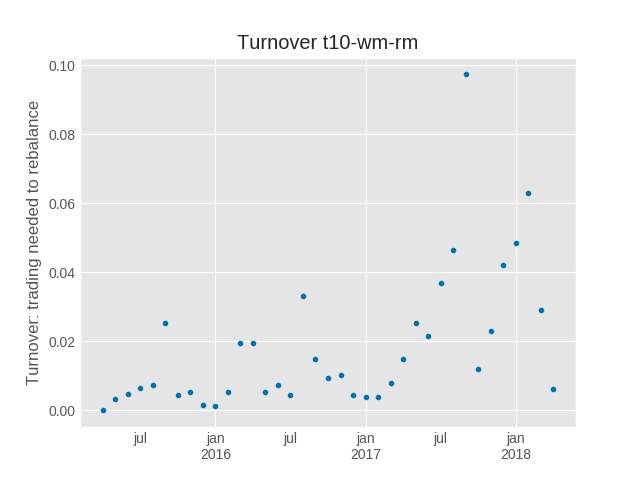
\includegraphics{/home/he2/Documents/crinfu/output/bsk/wei/turnover_1.png}
\caption{this fig is incorrect. see todo section.}
\end{figure}

\subsection{Correlation matrix}\label{correlation-matrix}

\subsection{Rolling correlation}\label{rolling-correlation}

The correlation matrix looks different depending on which time period we
use. To mitigate this weakness, they can be accompanied by graphing the
correlation using a rolling window.

\subsection{Autocorrelation}\label{autocorrelation-1}

ACF\_bsk1 ACF\_btc

\subsection{Effect of caps and weight
floors}\label{effect-of-caps-and-weight-floors}

capsweight floors\_effect\_1\_alts

\subsection{Effect of smoothing}\label{effect-of-smoothing}

Close to none.

\end{document}
